\documentclass[a4paper]{article}
\usepackage{graphicx, booktabs, natbib}
\usepackage{keyval}
  \setkeys{Gin}{height=0.5\textheight,width=\textwidth,keepaspectratio=true}
\usepackage{float}
  \restylefloat{figure}

\usepackage[colorlinks]{hyperref}
\usepackage{hyperxmp}

\hypersetup{
pdftitle={``Soap plants''---A proof of concept},
pdfauthor={Mohanadas Harish Chandar},
pdfcopyright={This work is licensed under a Creative Commons 
	      Attribution-Share Alike 3.0 Unported License.},
pdflicenseurl={http://creativecommons.org/licenses/by-sa/3.0/},
linkcolor={blue}, % Internal Links
anchorcolor={blue},
citecolor={blue},
filecolor={blue},
urlcolor={blue}
}

%% Font selection
%\renewcommand{\rmdefault}{ugm} %% URW Garamond No8
\usepackage{bera} %% Bitstream Vera for typewriter font
\usepackage{charter} %% Bitstream Charter for text fonts
%\usepackage[charter]{mathdesign} %% Matching MathDesign math fonts
%\usepackage[T1]{fontenc} 
%\renewcommand{\ttdefault}{fvm}
%\usepackage{ccfonts}

\title{``Soap plants''---A proof of concept}
\author{Mohanadas Harish Chandar}

\begin{document}
\maketitle
\section*{Introduction}
Jack,\footnote{Jack Sim, founder of the World Toilet Organisation} 
at a youth conference for social change,\footnotemark\ explained that 
poor people living in unsanitary conditions were not yet prepared to 
spend money on buying soap.

\footnotetext{SYINConnect `08: A conference on social change, 
              26th July 2008, Republic Polytechnic, Singapore}

He envisioned that if there were ``soap plants''---plants that could be 
directly used as soap substitures---grown near their washing areas,
sanitary conditions could be greatly improved.

This document aims to be a simple proof of concept of this vision,
and attempts to give examples of ``soap plants'' from around the world.
Most of the data was gathered from \citep{PFAF} and \citep{USDA}.

\section{Soapnut/Soapberry}
\begin{figure}[H]
\centering
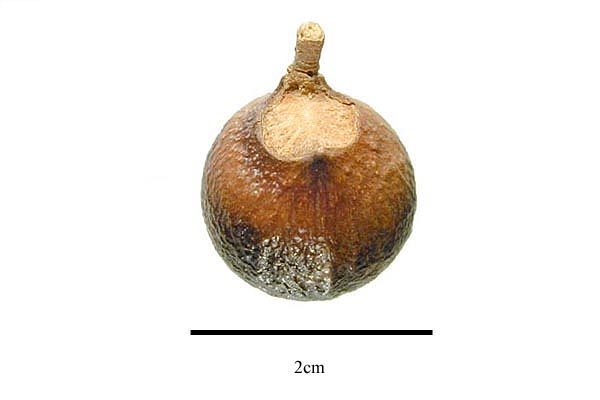
\includegraphics{images/sapindus_saponaria_fruit}
\caption{Fruit of {\it Sapinudus saponaria} \citep{Gibbons2006}.
         Rubbing in water produces lather.} 
\end{figure}

Soapnut or Soapberry, genus {\it Sapindus}, are shrubs or small trees found in 
warm temperate to tropical regions in the Americas and Asia. 
The fruit and seeds can be crushed or rubbed in water and used as soap.
It is commonly used for washing clothes.

\begin{figure}[H]
\centering
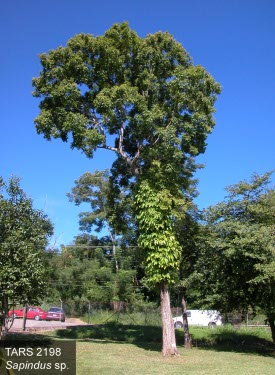
\includegraphics{images/sapindus_saponaria_tree}
\caption{Tree of {\it Sapinudus saponaria} \citep{USDA}. 
         It is found in the western hemisphere.} 
\end{figure}

\begin{table}[H]
\centering
\begin{tabular}{llll} \toprule
Family & Species & Distribution \\ \midrule
Sapindaceae & {\it Sapindus mukorossi} & China, Eastern Asia, \\
            &                          & Indian Subcontinent, Indo-China \\
            & {\it Sapindus rarak}     & China, Indian Subcontinent, \\
            &                          & Indo-China, Malesia \\
            & {\it Sapindus saponaria} & Southeastern USA, \\
            &                          & Mesoamerica, Caribbean, \\
            &                          & South America \\
            & {\it Sapindus trifoliatus} & Indian Subcontinent \\
\bottomrule
\end{tabular}
\caption{Distribution for several species of Soapnut/Soapberry.}
\end{table}

\clearpage
\section{Soapbark tree/Panama wood}

Soapbark tree or Panama Wood, {\it Quillaja saponaria}, is a species of
evergreen trees found in Chile and Peru. 
The fresh or dried inner bark can be used as a soap substitute.
It is an effective and gentle cleaner used for cleaning textiles
and the skin. 

\begin{figure}[H]
\centering
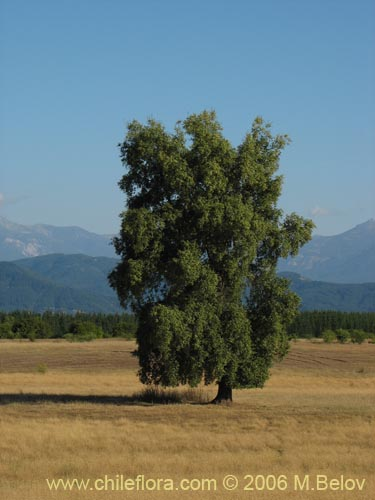
\includegraphics{images/quillaja_saponaria_tree}
\caption{Tree of {\it Quillaja saponaria} \citep{Belov2006}.
         It is found in Chile and Peru.} 
\end{figure}

\clearpage
\section{Yucca}
Yucca is a genus consisting of several species of
perennials, shrubs and trees. Common names for individual species include
Soaptree Yucca, {\it Yucca elata}, and Spanish Bayonet, 
{\it Yucca alifolia} or {\it Yucca baccata}. Yucca is native to
North America.

The roots can be crushed and soaked in water to 
release the suds for use as a soap. It is a good 
hair wash and can be used on the body and for washing clothes.

\begin{figure}[H]
\centering
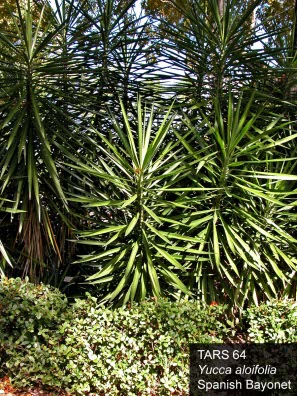
\includegraphics{images/yucca_alifolia_shrub}
\caption{Shrub of {\it Yucca alifolia} \citep{USDA}.
         It is found in USA, Mexico and Southern Europe} 
\end{figure}

\begin{table}[H]
\centering
\begin{tabular}{llll} \toprule
Family & Species & Distribution \\ \midrule
Agavaceae & {\it Yucca elata}    & USA, Mexico \\
          & {\it Yucca baccata}  & USA, Mexico \\
          & {\it Yucca alifolia} & USA, Mexico and Southern Europe \\
\bottomrule
\end{tabular}
\caption{Distribution for several species of {\it Yucca}.}
\end{table}

\clearpage
\section{Soapworts}
\begin{figure}[H]
\centering
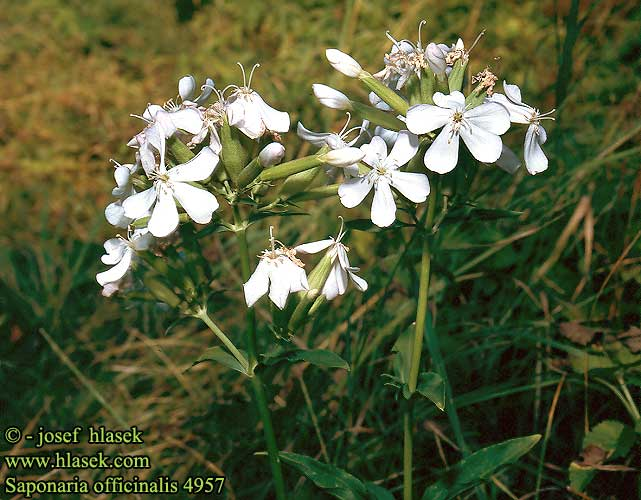
\includegraphics{images/saponaria_officinalis_plant}
\caption{{\it Saponaria officinalis} \citep{Hlasek}. 
         The whole plant can be heated in water to obtain a soap.} 
\end{figure}

Soapworts, genus {\it Saponaria}, are perennial herbs native to 
Europe and Southwest Asia. Soap can can be obtained by 
boiling/simmering the whole plant in water. 
The leaves and roots may contain higher concentrations of saponins.
Soapworts are commonly used as a effective but 
gentle cleaner for delicate fabrics.

\begin{table}[H]
\centering
\begin{tabular}{llll} \toprule
Family & Species & Distribution \\ \midrule
Caryophyllaceae & {\it Saponaria officinalis} & Southern Europe, \\
                &                             & Southwest Asia \\
                & {\it Saponaria ocymoides}   & Europe \\
\bottomrule
\end{tabular}
\caption{Distribution for several species of Soapworts.}
\end{table}


\clearpage
\bibliographystyle{plainnat}
\bibliography{references}

\section*{Copyright}
This work is licenced under the Creative Commons Attribution 
ShareAlike 3.0 License. 
You are free to share and remix this work under the conditions that you 
appropriately attribute it and that you distribute derivative works 
only under a license similar to this one.

To view a copy of this license, please visit 
\url{http://creativecommons.org/licenses/by-sa/3.0/} or write to
Creative Commons, 559 Nathan Abbott Way, Stanford, California 94305, USA.

You may contact me at 
\href{mailto:harishcms@email.com}{\tt harishcms@email.com} 
for the \LaTeX\ source and image files.
All images are copyright their respective owners. 

\begin{center}

\includegraphics[width=0.3\textwidth]{images/cc_by_sa}
\end{center}

\end{document}
